\documentclass[12pt]{article}
\usepackage{amsmath}
\usepackage{float}
\usepackage{algorithm}
\usepackage{amssymb}
\usepackage{graphicx}
\usepackage{hyperref}
\usepackage{cleveref}
\usepackage[most]{tcolorbox}
\usepackage[utf8]{inputenc}
\usepackage{tikz}
\usepackage{pstricks-add}
\usepackage{centernot}
\usepackage{algpseudocode}
\usepackage{enumerate}
\usepackage{MnSymbol}
\usepackage{mathtools}
\usepackage{subcaption}
\usepackage{geometry}
 \geometry{
 a4paper,
 total={170mm,257mm},
 left=20mm,
 top=20mm,
 }
\DeclarePairedDelimiter\ceil{\lceil}{\rceil}
\DeclarePairedDelimiter\floor{\lfloor}{\rfloor}
\DeclarePairedDelimiter\abs{\left|}{\right|}
\DeclareMathOperator{\arcsec}{arcsec}
\DeclareMathOperator{\arccot}{arccot}
\DeclareMathOperator{\arccsc}{arccsc}
\hypersetup{
    colorlinks=false,
    pdfborder={0 0 0},
}
\newcommand\tab[1][1cm]{\hspace*{#1}}
\newtheorem{theorem}{Theorem}
\newtheorem{corollary}{Corollary}
\usetikzlibrary{arrows,calc}
\title{MAT 1001: Calculus I}
\author{Alfonsus Rodriques Rendy}
\date{2021-11-18}

\begin{document}
\begin{center}
    \hspace*{-0.5cm}
    \framebox{
    \begin{minipage}{1\linewidth}
        \textbf{MAT1001 Calculus I} \\
        \vspace{-0.8cm}
        \begin{center}
            \huge{Lecture 17 - 20 : Transcendental Functions} 
            \\
            \vspace{0.5cm}
            \normalsize \textit{Lecture by Dr. Arjan Abeynaike} \\
            \vspace{0.3cm}
            \text{Scribe by Alfonsus Rodriques Rendy} \\
            \textrm{Nov 9, 2021 - Nov 18, 2021}
        \end{center}
    \end{minipage}}
\end{center}

\section{Differentiation of Inverse Functions}
\subsection{Type of Functions}
\paragraph{Definition} Let $f : D \rightarrow Y$ be a function.
\begin{itemize} 
    \item We say that $f$ is one-to-one (or \textbf{injective}) if $f(x_1) \neq f(x_2)$ for
    all distinct $x_1$ and $x_2$ in $D$ (that is, $x_1 \neq x_2$).
    \item We say that $f$ is onto (or \textbf{surjective}) if, for every $y \in Y$ , there
    exists $x \in D$ such that $f(x) = y$.
    \item We say that $f$ is \textbf{bijective} if it is both one-to-one and onto. A
    bijective function is called a bijection.
\end{itemize}

\paragraph{Example}
\begin{itemize} 
     \item $f : [0, 1] \to \mathbb{R}$, $f(x) = x^2$ is one-to-one function
     \item $f : [-1, 1] \to \mathbb{R}$, $f(x) = x^2$ is not one-to-one nor onto function
     \item $f : \mathbb{R} \to \mathbb{R}$, $f(x) = x + 1$ is bijective function
     \item $f : \mathbb{R} \to \mathbb{R}$, $f(x) = x^3$ is bijective function
     \item $f : \mathbb{R} \to [0, \infty]$, $f(x) = x^2$ is onto function
\end{itemize}

\paragraph{Remarks}
$f : D \to range(f)$ is always onto / surjective where range($f$) = $\{f(x) : x \in D \}$. By definition, every function
is onto its range. Therefore, $f : D \to range(f)$ is bijective if only if it is one-to-one, since $f$ is always onto.

\subsection{Inverse Function}
Let $f : D \to range(f)$ be one-to-one (bijective). The inverse function of $f$ is the function $f^{-1} : range(f) \to D$ defined by 
\[
    f^{ - 1} = x_0 \textrm{\tab where \tab} f(x_0) = y_0
\] 

Inverse of $f$ is only defined when $f : D \to range(f)$ is one-to-one (injective). Since $\forall \, x_0 \in D, \exists \, y_0 \in range(f)$ such that $f^{-1}(y_0) = x_0$,
we have $range(f^{-1}) = D$.

By definition:
\[
    \forall x_0 \in D, \textrm{\tab} (f^{-1} \circ f)(x_0) = f^{-1}(f(x_0)) = x_0
\]
and
\[
    \forall y_0 \in range(f), \textrm{\tab} (f \circ f^{-1})(y_0) = f(f^{-1}(y_0)) = y_0
\]
So $(f^{-1} \circ f)$ and $(f \circ f^{-1})$ are both identity function (a function that maps an element back to itself)

If $f$ is monotonic on $D$ then $f$ is one-to-one on D, so $f^{-1} : range(f) \to D$ must exist.
\paragraph{Example 1} $f : [0, 2] \to [0, 4], f(x) = x^2$ has inverse $f^{-1} : [0,4] \to [0,2], f^{-1} = \sqrt{y}$
\paragraph{Example 2} $f : R \setminus \{0\} \to R \setminus \{0\}, f(x) = \frac{1}{x}$ is the inverse of itself ($f^{-1} = f$) 
$f$ is not monotonic on $R \setminus \{0\}$ but is monotonic on $(-\infty, 0)$ and on $(0, \infty)$ separately.
\begin{figure}[H]
    \centering
    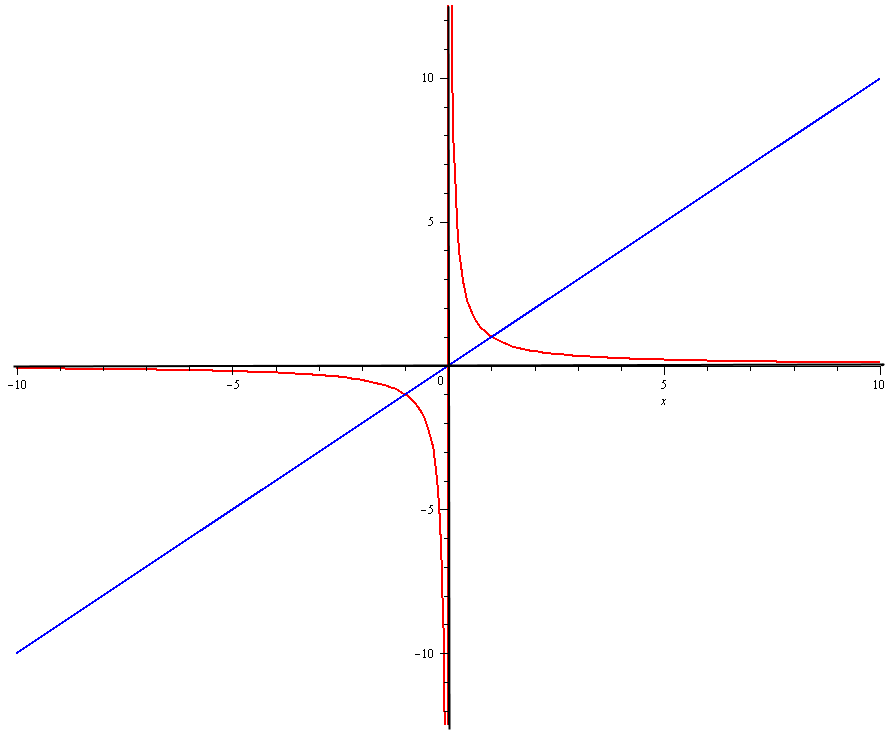
\includegraphics[width = 0.4\linewidth]{Images/graph of 1perx.png}
    \caption{The graph of $1/x$, it is the inverse function of itself}
\end{figure}

Several facts we will take for granted (no proof given)
\begin{itemize} 
     \item If $f$ is continuous and $f^{-1}$ exists, then $f^{-1}$ is also continuous.
     \item If $f$ is continuous and its domain is an interval, then $range(f)$ is also an interval
     \item If $f$ is one-to-one and continuous on an interval $I$ then $f$ is monotonic on $I$
\end{itemize}

\begin{theorem}[Derivative rule for inverses]
     Let $f : I \to Y$ be bijective where $I$ is an interval and $Y = range(f)$. If $f$ is differentiable and $f'$ is never zero on $I$
     then $f^{-1}$ is differentiable and
     \[
         (f^{-1}(y_0)) = \frac{1}{f'(f^{-1}(y_0))}
     \]
     for all $y_0 \in Y$, or if $f(x_0) = y_0$, 
     \[
         (f^{-1})'(f(x_0)) = \frac{1}{f'(x_0)}
     \]
\end{theorem}

\paragraph{Proof}
By fact 2, for $f : I \to Y$ where $I$ is an interval, $Y$ is also an interval. \\
Let $y_0 \in Y$ and let $x_0 \in I$ be such that $f(x_0) = y_0$. \\
For any $y_0 + h \in Y$ there is a unique $x_0 + k \in I$ such that
\[
    f(x_0 + k) = y_0 + h
\]
Note that
\[
    \lim_{h \to 0} \frac{f^{ - 1}(y_0 + h) - f^{-1}(y_0)}{h} = \lim_{h \to 0} \frac{x_0 + k - x_0}{f(x_0 + k) - y_0} 
\]
Since $f(x_0 + k) = y_0 + h$, we have
\[
    x_0 + k = f^{-1} (y_0 + h)
\]
By the fact 1, $f^{-1}$ is also continuous, So
\[
    \lim_{h \to 0} f^{-1}(y_0 + h) = f^{-1}(\lim_{h \to 0} y_0 + h) = f^{-1}(y_0) = x_0
\]
This means as $h \to 0$, $x_0 + k \to x_0$ so $k \to 0$. Hence, we have
\[
    (f^{-1})'(y_0) = \lim_{k \to 0} \frac{k}{f(x_0 + k) - f(x_0)}
\]
By definition
\[
    f'(x_0) = \lim_{k \to 0} \frac{f(x_0 + k) - f(x_0)}{k} 
\]
So,
\[
    (f^{-1})'(y_0) = \frac{1}{f'(x_0)} = \frac{1}{f'(f^{-1}(y_0))}
\]

If we assume the differentiability of $f^{-1}$ then the formula can be easily derived from the chain rule:
\begin{align*} 
    \because \: f^{-1}(f(x)) = x \textrm{\tab} \forall \: x \in I \\
    \therefore \: (f^{-1})'(f(x_0)) \cdot f'(x_0) = 1 \\
    \Rightarrow f^{-1}(y_0) = \frac{1}{f'(x_0)} = \frac{1}{f'(f^{-1}(y_0))}
\end{align*}

\paragraph{Remark} If $y_0$ is an endpoint of $Y$, then we may consider one-sided derivative instead.

\subsection{Inverse Function Examples}
\paragraph{Inverse of sine function}
Let $y_0 \in (-1, 1)$ and $x_0 \in \left(-\frac{\pi}{2}, \frac{\pi}{2} \right)$ be such that 
\[
    \sin x_0 = y_0
\]
Then by inverse differentiation
\[
    \arcsin '(y_0) = \frac{1}{\sin '(x_0)} = \frac{1}{\cos x_0} = \frac{1}{\sqrt{1 - \sin^2 x_0}} = \frac{1}{1 - y_0^2}
\]

If $y_0 = \pm 1$, then $x_0 = \pm \frac{\pi}{2}$ so $\sin'(x_0) = \cos x_0 = 0$ and the rule does not apply as the denominator is 0. from
geometric perspective, there are vertical tangent lines at $y_0 = \pm 1$ so the derivative do not exist as real numbers.

\paragraph{Inverse of ln function}
If $exp : \mathbb{R} \to (0, \infty)$ is the function $exp(x) = e^x$, then it has an inverse function
\[
    \ln : (0, \infty) \to \mathbb{R}
\]
that is called the natural logarithmic function.
Let $y_0 \in (0, \infty)$. By inverse differentiation, if $\exp(x_0) = y_0$ then
\[
    \ln'(y_0) = \frac{1}{\exp'(x_0)} = \frac{1}{\exp(x_0)} = \frac{1}{y_0}
\]
Hence
\[
    \frac{d}{dx} \ln(x) = \frac{1}{x} \textrm{\tab} \forall \, x \in (0, \infty)
\]

\subsection{Inverse Trigonometric Function}
Since trigonometric functions are not one-to-one, so its domain must be restricted to an interval $I$. 
\begin{figure}[H] 
     \centering
     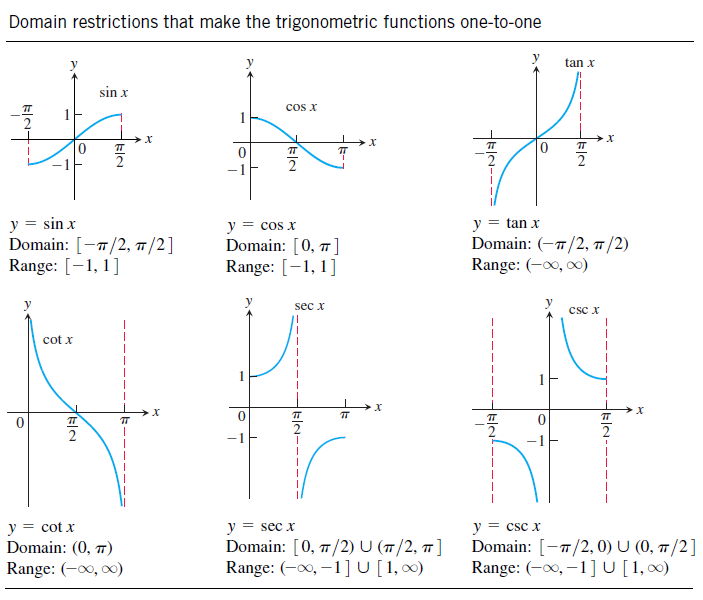
\includegraphics[width = 0.6\linewidth]{Images/trigonometric domain restricted.png}
     \caption{Trigonometric Functions with Restricted Domain}
\end{figure}

The inverse function can be obtained by reflecting the graph through the line $y = x$
\begin{figure}[H] 
    \centering
    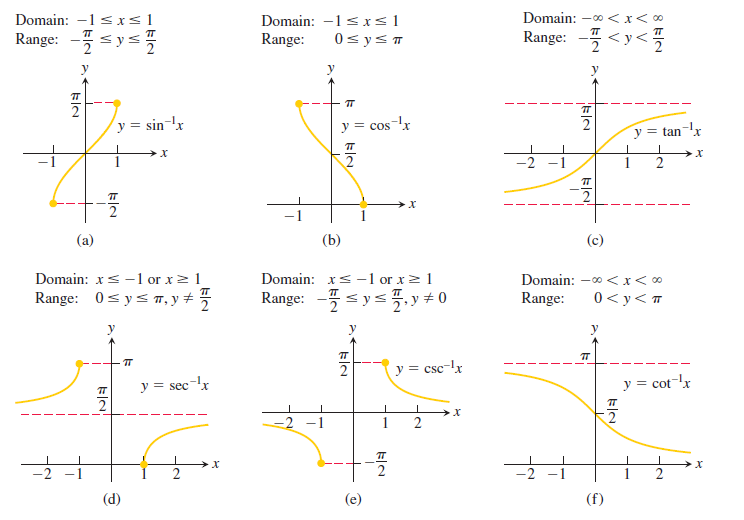
\includegraphics[width = 0.6\linewidth]{Images/inverse trigonometric function.png}
    \caption{Graph of inverse trigonometric functions}
\end{figure}

\paragraph{Inverse of $\tan x$} $\tan : \left( \frac{-\pi}{2}, \frac{\pi}{2} \right) \to \mathbb{R}$, $\arctan : \mathbb{R} \to \left( \frac{-\pi}{2}, \frac{\pi}{2} \right)$ \\ 
If $\arctan x_0 = y_0$ then $\tan y_0 = x_0$. By derivative rule for inverse function, we have
\[
    \arctan '(x_0) = \frac{1}{\tan'y_0} = \frac{1}{\sec^2 y_0} = \frac{1}{1 + \tan^2 y_0} = \frac{1}{1 + x_0^2}
\]

\paragraph{Inverse of $\sec x$} $\sec : \left[ 0,\frac{\pi}{2}\right) \cup \left(\frac{\pi}{2}, \pi \right) \to [1, \infty) \cup (-\infty, -1]$ 
$\arcsec : [1, \infty) \cup (-\infty, -1] \to \left[ 0,\frac{\pi}{2}\right) \cup \left(\frac{\pi}{2}, \pi \right)$

If $\arcsec x_0 = y_0$, $x_0 \neq \pm 1$, then 
\[
    \arcsec '(x_0) = \frac{1}{\sec 'y_0} = \frac{1}{\sec y_0 \tan y_0} = \frac{1}{x_0 \tan y_0} 
\]
Since $\sec^2 y_0 = 1 + \tan^2 y_0$
\[
    \tan y_0 = 
    \begin{cases} 
        \sqrt{\sec^2 y_0 - 1} & y_0 \in \left( 0, \frac{\pi}{2} \right) \\
        - \sqrt{\sec^2 y_0 - 1} & y_0 \in \left(\frac{\pi}{2}, \pi \right)
    \end{cases} 
\]
hence
\[
    \tan y_0 = 
    \begin{cases} 
        \sqrt{x_0^2 - 1} & x_0 > 1\\
        - \sqrt{x_0^2 - 1} & x_0 < - 1
    \end{cases} 
\]
Then,
\[
    \arcsec '\, x_0 = 
    \begin{cases} 
        \frac{1}{x_0 \sqrt{x_0^2 - 1}} & x_0 > 1\\
        \frac{1}{ - x_0 \sqrt{x_0^2 - 1}} & x_0 < - 1
    \end{cases} = \frac{1}{|x_0| \sqrt{x_0^2 - 1}}
\]

For other trigonometric function. We can derive it from the trigonometric identity: \\
Since $\sin y = \cos (y - \pi/2) = \cos (\pi/2 - y)$. If $x = \sin y$ then 
\[
    \arcsin x = y \textrm{\tab and \tab} \arccos x = \frac{\pi}{2} - y
\]
Then 
\[
    \arcsin x + \arccos x = \frac{\pi}{2}
\]
We can also show other identity:
\[
    \arctan x + \arccot  x = \frac{\pi}{2}
\]
\[
    \arcsec x + \arccsc  x = \frac{\pi}{2}
\]

\begin{figure}[H]
     \centering
     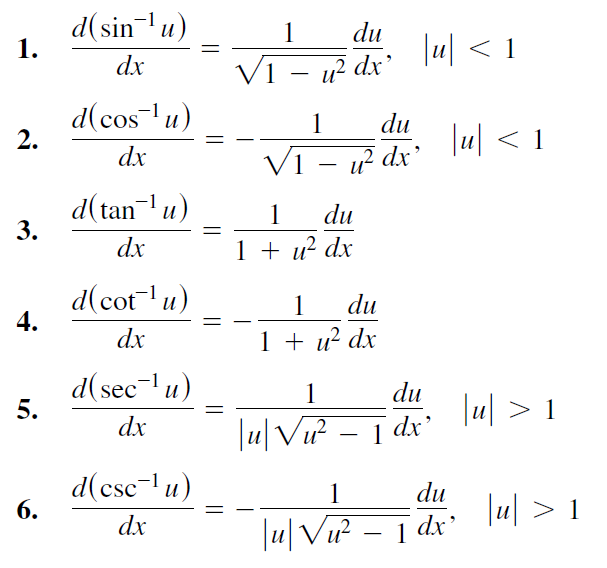
\includegraphics[width = 0.5 \linewidth]{Images/inverse trigonometric derivatives.png} 
     \caption{Derivatives of inverse trigonometric functions}
\end{figure}

\begin{figure}[H]
    \centering
    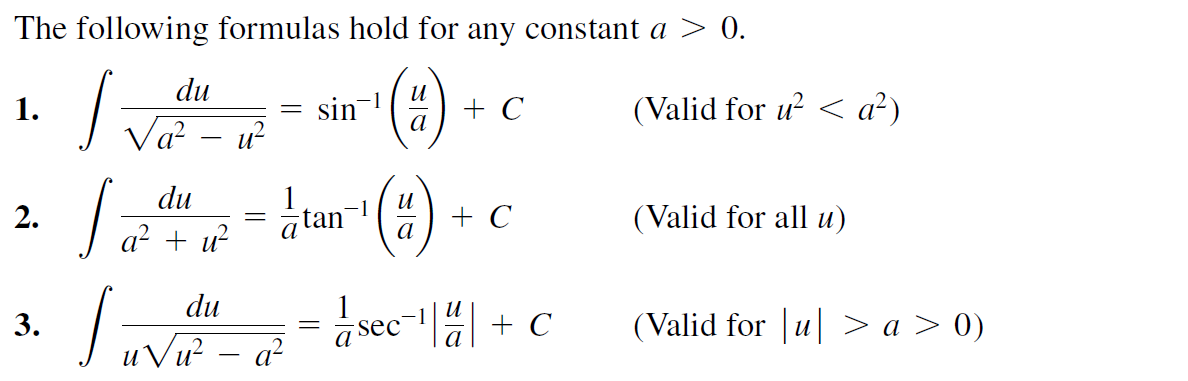
\includegraphics[width = 0.8 \linewidth]{Images/integral of inverse function.png} 
    \caption{Integral of inverse trigonometric functions}
\end{figure}
\section{Natural Logarithmic Function}
\subsection{Defining $e$}
\paragraph{Definition}
We define $\ln$ with domain $(0, \infty)$ by
\[
    \ln(x) = \int_1^x \frac{1}{t}\: dt
\]

\paragraph{Properties of natural logarithm}
\begin{itemize} 
     \item $\ln 1$ = 0 since $\int_1^1 \frac{1}{t}\: dt$ = 0
     \item $\frac{d}{dx} \ln(x)$ = $\frac{1}{x}$ (by FTC 1)
\end{itemize}

By those properties, ln is differentiable and hence continous on $(0, \infty)$. Since $\ln'(x) = \frac{1}{x} > 0 \: \forall \, x \in(0, \infty)$
ln is increasing on $(0, \infty)$. \\
Note that
\[
    \ln 4\, = \int_1^4 \frac{1}{t} \: dt = \int_1^2 \frac{1}{t} \: dt \int_2^3 \frac{1}{t} \: dt + \int_3^4 \frac{1}{t} \: dt \geq \frac{1}{2} + \frac{1}{3} + \frac{1}{4} > 1
\]
since $1/2, 1/3, 1/4$ is the minimum value of $\frac{1}{x}$ in the interval (by min-max inequality of integral).
Hence, by IVT, since $\ln$ is increasing, $\ln(1) = 0$ and $\ln(4) > 1$, there exists $x_0$ such that $\ln(x_0) = 0$ (with $x_0 \in (1, 4)$)
\paragraph{Definition : Euler's Number}
We define $e$ to be the unique number in $(0, \infty)$ such that $\ln(e) = 1$
\subsection{Algebraic Properties}
\begin{theorem}[Algebraic properties of ln]
    For any $b \in \mathbb{R}_{>0}$ and $x \in \mathbb{R}_{>0}$
    \begin{enumerate} 
         \item $\ln(bx) = \ln(b) + \ln(x)$
         \item $\ln(\frac{b}{x}) = \ln(b) - \ln(x)$
         \item $\ln(\frac{1}{x}) = - \ln(x)$
         \item $\ln(x^r) = r \ln(x)$ for any $r \in \mathbb{Q}$
    \end{enumerate}
\end{theorem}

\paragraph{Proof 1}
Let $f(x) = \ln(bx)$, defined on $(0, \infty)$. Then 
\[
    f'(x) = \frac{b}{bx} = \frac{1}{x} = \ln'(x)
\]
So, $f(x) = \ln(x) + C$ for some constant $C$, $\forall \, x \in (0, \infty)$. Since it must holds for
all $x$, let $x = 1$
\[
    \ln(b) = f(1) = \ln(1) + C = C
\]
Hence, $f(x) = \ln(bx) = \ln(x) + \ln(b)$

\paragraph{Proof 4}
Let $f(x) = \ln(x^r)$, defined on $(0, \infty)$ then 
\[
    f'(x) = \frac{rx^{r - 1}}{x^r} = \frac{r}{x} = \frac{d}{dx} r \ln(x)
\]
So, $f(x) = r \ln(x) + C$ for some constant $C$, $\forall \, x \in (0, \infty)$
Since it must holds for all $x$, let $x = 1$
\[
    f(1) = \ln(1^r) = 0 = r \ln(1) + C = C
\]
So, $C = 0$, and $\ln(x^r) = f(x) = r \ln(x)$

\paragraph{Proof 2}
Let $f(x) = \ln(b/x)$
\begin{align*} 
     \ln(\frac{b}{x}) &= \ln(bx^{-1}) \\
     &= \ln(b) + \ln(x^{-1}) \textrm{\tab by prop. 1}\\ 
     &= \ln(b) - \ln(x) \textrm{\tab by prop. 4} \\
\end{align*}

\paragraph{Proof 3}
Let $f(x) = \ln(1/x)$
\begin{align*} 
    \ln(\frac{1}{x}) &= \ln(1) - \ln(x) \textrm{\tab by prop. 2} \\
    &= - \ln(1)
\end{align*}

\subsection{Graph and Range}
\paragraph{Range} 
\[
    \ln(2) = \int_1^2 \frac{1}{t} \, dt > (2 - 1)(\frac{1}{2}) = \frac{1}{2}
\]
For any $n \in \mathbb{Z}_{+}$, 
\[
    \ln(2^n) = n \ln(2) > \frac{n}{2}
\]
Since ln is increasing, 
\[
    \ln(x) \geq \ln(x^n) > \frac{n}{2} \textrm{\tab} \forall \, x \in [2^n, \infty)
\]
So, as $n \to \infty$, $\ln(2^n) \to \infty$ and $\lim{x \to \infty} \ln(x) = \infty$
And for $x \to 0^{+}$
\[
    \lim_{x\to 0^{ +}} \stackrel{x = \frac{1}{u}}{=} \lim_{u \to \infty} \ln\left(\frac{1}{u}\right) = \lim_{u \to \infty} ( -\ln(u)) = -\infty
\]
Now let $y_0$ be any fixed real number. By two limits above, there exist $x_1$ and $x_2$ in $(0, \infty)$ such that
\[
    \ln(x_1) < y_0 \textrm{\tab and \tab} \ln(x_2) > y_0
\]
By IVT, there exists $c \in [x_1, x_2]$ such that $\ln c = y_0$. Hence, $range(\ln) = \mathbb{R}$

\paragraph{Concavity} Since
\[
    \ln''(x) = \frac{d}{dx} \frac{1}{x} = - \frac{1}{x^2} < 0 \textrm{\tab} \forall \, x \in (0, \infty)
\]
the curve $y = \ln x$ is concave down.

\paragraph{Limits of derivatives}
Since
\[
    \lim_{x \to 0^{ +}} \ln'(x) = \lim_{x \to 0^{ +}} \frac{1}{x} = \infty
\]
and
\[
    \lim_{x \to \infty} \ln'(x) = \lim_{x \to \infty} \frac{1}{x} = 0 
\]
$y = \ln x$ tends to have a "flat-ish" tangent line as $x$ grows big, yet it is not bounded above.
\subsection{Composite function of $\ln(x)$}
Let $g: D \to R_{>0}$ be differentiable on $D$. Then:
\[
    (\ln \circ g)'(x) = \ln'(g(x))g'(x) = \frac{g'(x)}{g(x)}
\]
If we take $g(x) = |x|$ with $D = \mathbb{R} \setminus {0}$, then 
\[
    g'(x) = 
    \begin{cases}
        1 & x > 0 \\
        - 1 & x < 0
    \end{cases} 
\]
so,
\[
    g'(x) = \frac{|x|}{x} 
\]
By the formula above, we have:
\[
    \frac{d}{dx} \ln |x| = \frac{g'(x)}{g(x)} = \frac{|x|}{x} \cdot \frac{1}{|x|} = \frac{1}{x}
\]
This means that for $x \in R \setminus{0}$, $\ln |x|$ is an antiderivative of $1/x$, 

\paragraph{The Integral of 1/x}
If $x$ is a differentiable function, and is never zero:
\[
    \int \frac{1}{x} \: = \ln |x| + C
\]

\noindent
More generally if $g(x) = |f(x)|$ where $f$ is differentiable and never zero, then by the chain rule 
\[
    g'(x) = \frac{|f(x)|}{f(x)} \cdot f'(x) 
\]
So, 
\[
    \frac{d}{dx} \ln |f(x)| = \frac{1}{|f(x)|} \cdot \frac{d}{dx} |f(x)| = \frac{f'(x)}{f(x)} 
\]

\paragraph{The Composite Integral of f'(x)/f(x)}
If $f(x)$ is differentiable and $f(x) \neq 0$
\[
    \int \frac{f'(x)}{f(x)} = \ln |f(x)| + C 
\]

\paragraph{Example 1} $\int \tan x \: dx$ and $\int \sec x \: dx$
\begin{align*} 
     \int \tan x \: dx &= \int \frac{\sin x}{\cos x} \\
     &= - \int \frac{ - \sin x}{\cos x} \: dx \\
     &= - \ln |\cos x| + C = \ln |\sec x| + C
\end{align*}
valids on where $\sec x \neq 0$
\begin{align*} 
    \int \sec x \: dx &= \int \sec x \frac{\sec x \tan x}{\sec x \tan x}  \\
    &= - \int \frac{\sec^2 x + \tan x \sec x}{\sec x + \tan x} \: dx \\
    &= \ln |\sec x + \tan x| + C
\end{align*}
valids on where $\sec x + \tan x \neq 0, \in \mathbb{R}$.

\paragraph{Integrals of tangent, cotangent, secant and cosecant}
\begin{itemize} 
     \item $\int \tan u \: du = \ln |\sec u| + C$
     \item $\int \cot u \: du = \ln |\sin u| + C$
     \item $\int \sec u \: du = \ln |\sec u + \tan u| + C$
     \item $\int \csc u \: du = - \ln |\csc u + \cot u| + C$
\end{itemize}

\paragraph{Example 2}
\[
    \int_0^{\frac{\pi}{6}} \tan 2x \: dx
\]
Let $u = 2x$
\begin{align*} 
    \int_0^{\frac{\pi}{6}} \tan 2x \: dx &= \int_0^{\frac{\pi}{3}} \tan u \frac{1}{2} \: du \\
    &= \frac{1}{2} \left[ \ln |\sec u| \right]_0^{\frac{\pi}{3}} \\
    &= \frac{1}{2} \ln \left|\frac{\sec \frac{\pi}{3}}{\sec 0} \right| \\ 
    &= \frac{1}{2} \ln 2 
\end{align*}

\subsection{Logarithmic differentiation}
Suppose $F(x)$ involves complicated products, quotients and powers, e.g.
\[
    F(x) = \frac{f_1(x)^{m_1}f_2(x)^{m_2}}{f_3(x)^{m_3}} 
\]
Takin ln on both sides we get:
\[
    \ln F(x) = m_1 \ln f_1(x) + m_2 \ln f_2(x) - m_3 \ln f_3(x)
\]
Differentiating both sides yields:
\[
    \frac{F'(x)}{F(x)} = m_1 \frac{f_1'(x)}{f_1(x)} + m_2 \frac{f_2'(x)}{f_2(x)} - m_3 {f_3'(x)}/f\frac{f_3'(x)}{f_3(x)}  
\]

\paragraph{Example} Find $y'$ where 
\[
  y = \frac{x^{\frac{3}{4}}\sqrt{x^2 + 1}}{(3x + 2)^5}
\]
\begin{align*} 
    \ln y &= \frac{3}{4} \ln x + \frac{1}{2} \ln (x^2 + 1) - 5 \ln (3x + 2) \\
    \frac{y'}{y} &= \frac{3}{4} \frac{1}{x} + \frac{1}{2} \frac{2x}{x^2 + 1} - 5 \frac{3}{3x + 2} \\
    y' &= \frac{x^{\frac{3}{4}}\sqrt{x^2 + 1}}{(3x + 2)^5} \left( \frac{3}{4x} + \frac{x}{x^2 + 1} - \frac{15}{3x + 2}  \right)
\end{align*}
\section{Natural Exponential Function}
\subsection{Definition}
Since $\ln : (0, \infty) \to \mathbb{R}$ is bijective, it has an inverse function
\[
    \exp : \mathbb{R} \to (0, \infty)
\]
called the natural exponential function. \\
Since $\ln e = 1$ by definition, we have $e = \exp(1)$.
Since $e > 0$, $e^r$ is defined for any rational power $r$, we have
\[
    \exp(r) = e^r, \textrm{\tab} \forall \, r \in \mathbb{Q}
\]
For irrrational power $x$ we simply define $e^x$ as follows:
\[
    e^x = \exp{x}, \textrm{\tab} \forall \, x \in \mathbb{R} \setminus \mathbb{Q}
\]
Consequently:
\[
    e^{\ln x} \textrm{\tab} \forall \, x \in (0, \infty)
\]
\[
    \ln (e^x) = x , \textrm{\tab} \forall \, x \in \mathbb{R}
\]
Since ln is differentiable and $\ln'$ is never zero, by derivative rule for inverse function,
$\exp$ is also differentiable. Let $y = \exp{x}$ then $\ln y = x$
\begin{align*} 
    \frac{1}{y} \cdot \frac{dy}{dx} &= 1 \\
    \frac{dy}{dx} &= y = \exp (x)
\end{align*}

\paragraph{Integral of $e^x$}
\[
    \exp'(x) = \exp(x) \textrm{\tab or \tab} \frac{d}{dx} e^x = e^x \textrm{\tab and \tab} \int e^x = e^x + C
\]

\paragraph{Example 1} $\frac{d}{dx} e^{\sqrt{3x + 1}}$
\begin{align*} 
    \frac{d}{dx} e^{\sqrt{3x + 1}} &= e^{\sqrt{3x + 1}} \cdot \frac{d}{dx} \sqrt{3x + 1} \\
    &= e^{\sqrt{3x + 1}} \cdot \frac{1}{2} (3x + 1)^{ \frac{1}{2}} \cdot 3 \\
\end{align*}

\paragraph{Example 2} Find
\[
    \int_0^{\frac{\pi}{2}} e^{\sin x} \cos x \: dx
\]
Let $u = \sin x$,

\begin{align*} 
    \int_0^{\frac{\pi}{2}} e^{\sin x} \cos x \: dx &= \int_0^1 e^u \: du \\
    &= e^1 - e^0 = e - 1
\end{align*}

\subsection{Algebraic Properties}
\begin{theorem}[Algebraic Properties of $e^x$]
    For any real number $x_1, x_2$ and $x$:
    \begin{enumerate} 
         \item $e^{x_1}e^{x_2} = e^{x_1 + x_2}$
         \item $e^{-x} = 1/e^x$
         \item $e^{x_1}/e^{x_2} = e^{x_1 - x_2}$
         \item $(e^x)^r = e^{rx}, \forall \, r \in \mathbb{Q}$
    \end{enumerate}
\end{theorem}

\paragraph{Proof 1}
Let $y_1 = e^{x_1}, y_2 = e^{x_2}$. then
\begin{align*} 
    e^{x_1 + x_2} &= e^{\ln y_1 + \ln y_2} \\
    &= e^{\ln y_1 y_2} \\
    &= y_1y_2 = e^{x_1}e^{x_2}
\end{align*}

\paragraph{Proof 4}
Let $y = e^x$. Then
\[
    e^{rx} = e^{r \ln y} = e^{\ln y^r} = y^r = (e^x)^r
\]

\paragraph{Proof 3}
\begin{align*} 
    e^{x_1 - x_2} &= e^{x_1}e^{ - x_2} \\
    &= e^{x_1}(e^{x_2})^{ - 1} \\
    &= \frac{e^{x_1}}{e^{x_2}}
\end{align*}

\paragraph{Proof 2}
\begin{align*} 
    e^{ - x} &= e^{0 - x} \\
    &= \frac{e^0}{e^x} = \frac{1}{e^x}
\end{align*}

\section{General Power and Exponential Functions}
With $e^x$ defined for all $x \in \mathbb{R}$, we can now define $a^x$ for any $a \in (0, \infty)$ and $x \in \mathbb{R}$
\paragraph{Definition}
For any $a \in (0, \infty)$ and $x \in \mathbb{R}$ we define
\[
    a^x = e^{x \ln a}
\]
When $a = e$, we have $a^x = e^{x \ln a} = e^{x \ln e} = e^x$

\paragraph{Definition: General Exponential Function with base a}
Fix $a \in (0, \infty)$. Define $f(x) = a^x$, $D = \mathbb{R}$

\paragraph{Definition: General Power Function}
Fix $a \in \mathbb{R}$. Define $f(x) = x^a$, $D = (0, \infty)$. 
\[
    x^a = e^{a \ln x}
\]

The algebraic propety for $\ln$ and $\exp$ also holds for irrational values of $r$:
\begin{enumerate}
    \item $\ln {x^a} = a \ln x$, $\forall \, x \in (0, \infty)$, $\forall \, a \in \mathbb{R}$
    \item $(e^x)^a = e^{ax}$, $\forall \, x \in \mathbb{R}$, $\forall \, a \in \mathbb{R}$
\end{enumerate}
(1) holds because $e^{\ln (x^a)} = x^a = e^{a \ln x}$
(2) can be shown using (1), $x^a = \ln(e^{x})^a = a \ln(e^x) = ax$

\subsection{Algebraic Properties}
\begin{theorem}[Algebraic Properties of $a^x$]
    For $a \in (0, \infty)$ and anyreal number $x_1, x_2$, $x$, and $r$:
    \begin{enumerate} 
         \item $a^{x_1}e^{x_2} = a^{x_1 + x_2}$
         \item $a^{-x} = 1/a^x$
         \item $a^{x_1}/a^{x_2} = a^{x_1 - x_2}$
         \item $(a^x)^r = a^{rx}$
    \end{enumerate}
\end{theorem}

\paragraph{Proof 1} 
\begin{align*} 
     a^{x_1 + x_2} &= e^{(x_1 + x_2)\ln a} \\
     &= e^{x_1 \ln a + x_2 \ln a} \\
     &= e^{x_1\ln a}e^{x_2\ln a} \\
     &= a^{x_1}a^{x_2}
\end{align*}

\subsection{General Power Rule}
\begin{theorem}[General Power Rule for Differentiation]
    \[
        \frac{d}{dx} x^a = ax^{a - 1}, \textrm{\tab} \forall \, x \in (0, \infty)
    \]
\end{theorem}

\paragraph{Proof}
\begin{align*} 
    \frac{d}{dx} x^a &= \frac{d}{dx} e^{a \ln x} \\
    &= e^{a \ln x} a \frac{d}{dx} \ln (x) \\
    &= e^{a \ln x} \frac{a}{x} \\
    &= x^a\cdot \frac{a}{x} = ax^{a - 1}
\end{align*}

\paragraph{Example 1} If $f(x) = x^x \: \forall \, x \in (0, \infty)$, what is $f'(x)$?
\[
    f(x) = x^x = e^{x \ln x}
\]
So, 
\begin{align*} 
    f'(x) &= e^{x \ln x} \left( x \cdot \frac{1}{x} + 1 \ln x \right) \\
    &= e^{x \ln x} (1 + \ln x) \\
    &= x^x (1 + \ln x)
\end{align*}

\subsection{Finding e}
\begin{theorem}[Limit of $e$]
    \[
        e = \lim_{x \to 0} (1 + x)^{\frac{1}{x}}
    \]
\end{theorem}

\paragraph{Proof}
\[
    (1 + x)^{\frac{1}{x}} = e^{\frac{1}{x} \ln (1 + x)}, \textrm{\tab} \forall \, x \in (-1, 1) \setminus \{0\}
\]
So, by continuity of exp function, we have
\[
    \lim_{x \to 0} (1 + x)^{\frac{1}{x}} = \lim_{x \to 0} e^{\frac{1}{x} \ln (1 + x)} = e^{\lim_{x \to 0} \frac{1}{x} \ln (1 + x)}
\]
Now the value of the limit is:
\[
    \lim_{x \to 0} \frac{1}{x} \ln (1 + x) = \lim_{x \to 0} \frac{(\ln(1 + x) - \ln (1))}{x} = \ln'(1) = 1 
\]
Hence
\[
    \lim_{x \to 0} (1 + x)^{\frac{1}{x}} = e^1 = e
\]
By looking at the value of $(1 + x)^{1/x}$, we get $e \approx 2.718281823845$

\subsection{Derivative and Graphs}
For a fixed $a \in (0, \infty)$, let $f(x) = a^x$, then $f(x) = e^{x \ln a}$, so
\[
    f'(x) = e^{x \ln a} \ln a = a^x \ln a
\]

\paragraph{Derivative of $a^x$} For a fixed $a \in (0, \infty)$ we have
\[
    \frac{d}{dx} a^x = a^x \ln a
\]

\paragraph{Integral of $a^x$} Provided that $a \neq 1$, we have
\[
    \int a^x dx = \frac{a^x}{\ln a} + C
\]

Note that 
\begin{align*} 
     \frac{d}{dx} a^x 
     \begin{cases} 
        > 0 \: \forall \, x & a > 1 \\
        < 0 \: \forall \, x & 0 < a < 1 \\
     \end{cases} 
\end{align*}
So $f(x) = a^x$ is increasing on $\mathbb{R}$ if $a > 1$ and decreasing on $\mathbb{R}$ if $0 < a < 1$

\begin{figure}[H]
     \centering
     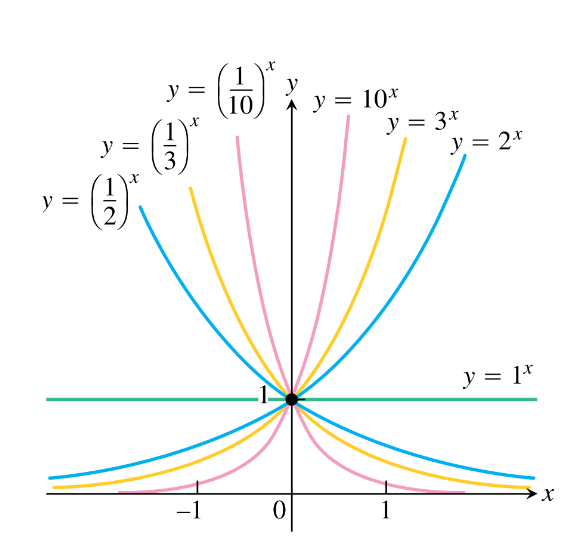
\includegraphics[width = 0.4 \linewidth]{Images/general exponential func.png}
     \caption{Graph of $a^x$}
\end{figure}

Since $f''(x) = (\ln a)^2 a^x > 0$, $y = a^x$ is always concave up on $\mathbb{R}$
\section{General Logarithmic Functions}
\subsection{Algebraic Properties}
Fix $a \in (0, \infty) \setminus\{1\}$. The function $f_a$ given $f_a(x) = a^x$ is monotonic, so it is one-to-one domain $\mathbb{R}$.
From the definition $a^x = e^{x \ln a}$ and the fact that range(exp) = $(0, \infty)$, it follows that range of $f_a$ is also $(0, \infty)$. Hence,
$f_a : \mathbb{R} \to (0, \infty)$ has an inverse function $\log_a : (0, \infty) \to \mathbb{R}$ called the logarithmic function with base $a$.

\noindent
By definition,
\[
    a^{\log_a x} = x, \textrm{\tab} \forall \, x \in (0, \infty)
\]
and
\[
    \log_a a^x = x, \textrm{\tab} \forall \, x \in \mathbb{R}
\]

Since $a^{\log_a x} = x$, 
\[
    \ln a^{\log_a x} = \ln x
\]
So, 
\[
    \log_a x = \frac{\ln x}{\ln a} 
\]

Hence, with that identity, we can show that the algebraic properties for $\ln$ also hold for $\log_a$

\paragraph{Property 1}
\begin{align*} 
    \log_a xy &= \frac{\ln xy}{\ln a} \\
    &= \frac{\ln x + \ln y}{\ln a} \\
    &= \log_a x + \log_a y 
\end{align*}

\subsection{Derivatives}
From the identity $\log_a x = \ln x / \ln a$, we can see that
\[
    \frac{d}{dx} \log_a x = \frac{1}{x \ln a}
\]
\section{L'hospital's Rule}
\subsection{Rule and Examples}
In some cases, limit can takes the indeterminate forms, such as $0/0$ and $\infty/\infty$, for example:
\[
    \lim_{x \to 0} \frac{x - \sin x}{x^3} \textrm{\tab} \lim_{x \to \infty} \frac{\ln x}{x^2} 
\]

\begin{theorem}[L'Hospital's Rule]
     Let $c \in \mathbb{R}$, suppose that $f$ and $g$ are differentiable on 
     $D = (c - a, c + a)\setminus\{c\}$ for some $a > 0 $ and that $g'(x) \neq 0$ for all $x \in D$. Suppose
     that one of the two following conditions holds:
     \begin{itemize} 
          \item  $\lim_{x \to c} f(x) = \lim_{x \to c} g(x) = 0 $
          \item $\lim_{x \to c} f(x) \in \{-\infty, \infty\}$ and $\lim_{x \to c} g(x) \in \{-\infty, \infty\}$
     \end{itemize}
     Then 
     \[
         \lim_{x \to c} \frac{f(x)}{g(x)} = \lim_{x \to c} \frac{f'(x)}{g'(x)} 
     \]
     provided that the limit on the right exists (or is $\infty$ or $-\infty$)
\end{theorem}

\paragraph{Remarks}
L'Hospital's rule is also valid if we replace it with one-sided limit. If $D$ is changed to an unbounded interval, then L'Hospital's rule is also
valid if we replace it the limit $x \to c$ with $x \to \infty$ or $x \to - \infty$

\paragraph{Example 1} Show that
\[
    \lim_{x \to 1} \frac{x^3 + 3x - 4}{x^4 - 6x^2 + 5} = \frac{ -3}{4} 
\]
Since the limit take the form $0/0$, we can apply L'Hospital's Rule.
\begin{align*} 
    \lim_{x \to 1} \frac{x^3 + 3x - 4}{x^4 - 6x^2 + 5} &= \lim_{x \to 1} \frac{3x^2 + 3}{4x^3 - 12x} \\
    &= \frac{3 + 3}{4 - 12} =  \frac{ -3}{4} 
\end{align*}

\paragraph{Example 2} Show that
\[
    \lim_{x \to 0} \frac{x - \sin x}{x^3} = \frac{1}{6} 
\]
Since the limit take the form $0/0$, we can apply L'Hospital's Rule.
\begin{align*} 
    \lim_{x \to 0} \frac{x - \sin x}{x^3} = \lim_{x \to 0} \frac{\sin x}{6x} 
\end{align*}
Since it takes the form 0/0 again.
\begin{align*} 
    \lim_{x \to 0} \frac{\sin x}{6x} = \lim_{x \to 0} \frac{\cos x}{6} = \frac{1}{6} 
\end{align*}

\paragraph{Example 3} Show that
\[
    \lim_{x \to 0} \frac{\ln^3 (x + 1)}{e^x - x - 1} = 0 
\]
Since the limit take the form $0/0$, we can apply L'Hospital's Rule.
\begin{align*} 
    \lim_{x \to 0} \frac{\ln^3 (x + 1)}{e^x - x - 1} = \lim_{x \to 0} \frac{3 \ln^2(x + 1)}{(x + 1)(e^x - 1)} 
\end{align*}
Since it takes the form 0/0 again.
\begin{align*} 
    \lim_{x \to 0} \frac{3 \ln^2(x + 1)}{(e^x - 1)} = \lim_{x \to 0} \frac{6 \ln(x + 1)}{e^x (x + 1)}  = \frac{0}{1} = 0
\end{align*}

\paragraph{Example 4} Show that
\[
    \lim_{x \to 2} \frac{\sin (\pi x)}{(x - 2)^2} 
\]
does not exist.
Since the limit take the form $0/0$, we can apply L'Hospital's Rule.
\begin{align*} 
    \lim_{x \to 2} \frac{\sin (\pi x)}{(x - 2)^2} = \lim_{x \to 2} \frac{\pi \cos(\pi x)}{2(x - 2)} 
\end{align*}
Taking the left-hand limit we get $-\infty$ and the right hand limit is $\infty$, hence the limit does not exist.

\paragraph{Example 4} Show that
\[
    \lim_{x \to \infty} \frac{\ln x}{x^\pi} = 0 
\]
Since the limit take the form $\infty/\infty$, we can apply L'Hospital's Rule.
\begin{align*} 
    \lim_{x \to \infty} \frac{\ln x}{x^\pi} = \lim_{x \to \infty} \frac{\frac{1}{x}}{\pi x^{\pi - 1}} =  \lim_{x \to \infty} \frac{1}{\pi x^\pi} = 0
\end{align*}

There are other indeterminate forms such as $\infty \cdot 0$, $1^{\infty}$, and $\infty - \infty$. By transforming such forms into
$0/0$ or $\pm \infty / \pm \infty$, L'Hospital's rule can be used.
\paragraph{Example 5} Show that
\[
    \lim_{x \to \infty} x^2 e^{ - \sqrt{x}} = 0
\]
The form is $\infty \cdot 0$
\begin{align*} 
    \lim_{x \to \infty} x^2 e^{ - \sqrt{x}} &= \lim_{x \to \infty} \frac{x^2}{e^{\sqrt{x}}} \\
    &= \lim_{x \to \infty} \frac{2x}{e^{\sqrt{x}} \frac{1}{2 \sqrt{x}}} = \lim_{x\to \infty} \frac{4x^{\frac{3}{2}}}{e^{\sqrt{x}}} \\
    &= \lim_{x \to \infty} \frac{6x^{\frac{1}{2}}}{e^{\sqrt{x}} \frac{1}{2 \sqrt{x}}} = \lim_{x \to \infty} \frac{12x}{e^{\sqrt{x}}} \\
    &= \lim_{x \to \infty} \frac{12}{e^{\sqrt{x}} \frac{1}{2 \sqrt{x}}} = \lim_{x \to \infty} \frac{24 \sqrt{x}}{e^{\sqrt{x}}} \\
    &= \lim_{x \to \infty} \frac{12}{\sqrt{x} e^{\sqrt{x}} \frac{1}{2 \sqrt{x}}} = \lim_{x \to \infty} \frac{24}{e^{\sqrt{x}}} = \frac{24}{\infty} = 0 
\end{align*}
\paragraph{Example 5} Show that
\[
    \lim_{x \to 0} (1 - 2x)^{\frac{3}{x}} = e^{- 6}
\]
The form is $1^{\infty}$

\begin{align*} 
    \lim_{x \to 0} (1 - 2x)^{\frac{3}{x}} &= e^{\frac{3}{x} \ln(1 -2x)} \\
    &= e^{\lim_{x \to 0} \frac{3}{x} \ln(1 - 2x)} \\
\end{align*}

\[
    \lim_{x \to 0} \frac{3}{x} \ln(1 - 2x) = \lim_{x \to 0} \frac{3}{1 - 2x} ( - 2) = - 6
\]
Hence,
\[
    \lim_{x \to 0} (1 - 2x)^{\frac{3}{x}} = e^{- 6}
\]

\paragraph{Example 5} Show that
\[
    \lim_{x \to 0} \frac{1}{x} - \frac{1}{\sin x} = 0
\]
The form is $\infty - \infty$
\begin{align*} 
    \lim_{x \to 0} \frac{1}{x} - \frac{1}{\sin x} &= \lim_{x \to 0} \frac{\sin x - x}{x \sin x}\, \
    &= \lim_{x \to 0} \frac{\cos x - 1}{\sin x + x \cos x} = \lim_{x \to 0} \frac{ - \sin x}{\cos x + \cos x - \sin x} = \frac{0}{2} = 0
\end{align*}

\subsection{L'Hospital's Limitations}
To apply L'Hospital's rule, make sure to stop at the right step, that is when the indeterminate forms do not occur anymore.
For example
\[
    \lim_{x \to 0} \frac{x^2}{x^2 + \sin x} = \lim_{x \to 0} \frac{2x}{2x + \cos x} = \lim_{x \to 0} \frac{2}{2 - \sin x} = \frac{2}{2} = 1 
\]
The second equality fails because the second limit does not satisfy the assumption of L'Hospital's rule.
\noindent
L'Hospital's rule has its limitation. For some limit, it will only go back to the original form. For example:
\[
    \lim_{x \to \infty} \frac{x^2 + \sin x}{x^2} \textrm{\tab} \lim_{x \to \infty} \frac{e^x - e^{-x}}{e^x + e^{-x}}\, 
\]
\subsection{Cauchy's Mean Value Theorem}
\begin{theorem}[Cauchy's Mean Value Theorem]
     Suppose $f$ and $g$ are continuous on $[a, b]$ and differentiable throughout $(a, b)$ and also suppose $g'(x) \neq 0$ throughout $(a, b)$. Then there exists $c \in (a, b)$ such that
     \[
         \frac{f'(c)}{g'(c)} = \frac{f(b) - f(a)}{g(b) - g(a)} 
     \]
\end{theorem}

\begin{figure}[H]
     \centering
     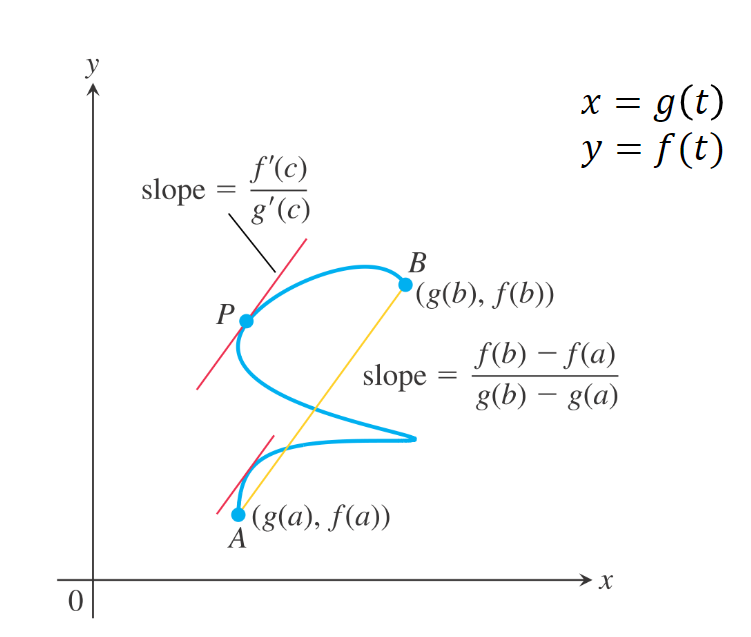
\includegraphics[width = 0.5\linewidth]{Images/cauchys MVT.png}
     \caption{There is at least one point $P$ on curve $C$ for which the slope of the tangent is the same as the secant joining $A$ and $B$}
\end{figure}

\paragraph{Proof}
Note that $g(b) \neq g(a)$, since by MVT
\[
    g(b) = g(a) + g'(c_0)(b - a), \textrm{\tab for some } c_0 \in (a, b)
\]
and we assume $g'(c_0) \neq 0$ (Rolle's Theorem). \\
Now define $h$ by 
\[
    h(t) = f(a) + \left(\frac{f(b) - f(a)}{g(b) - g(a)} \right)(g(t) - g(a)) - f(t)
\]
and note that $h(a) = 0 = h(b)$. Since $h$ is continuous on $[a, b]$ and differentiable on $(a, b)$, by 
Rolle's Theorem, there exists $c \in (a, b)$ such that $h'(c) = 0$ means:
\[
    \frac{f(b) - f(a)}{g(b) - g(a)} = \frac{f'(c)}{g'(c)} 
\]
\subsection{Proof of L'Hospital's Rule}
We will prove L'Hospital's rule for special case where: $f$ and $g$ are differentiable on $(c - a, c + a)$ for some $a > 0$,
$g'(x) \neq 0$, $\forall \, x \in (c- a, c + a)\setminus\{c\}$ and $\lim_{x \to c} f(x) = 0 = \lim_{x \to c} g(x)$

\noindent
First we will show for $\lim_{x \to c^+}$ Pick any $x \in (c - a, c + a)$ and consider Cauchy's MVT on $[c, x]$, there exists $x_0 \in (c, x)$ such that
\[
    \frac{f'(x_0)}{g'(x_0)} = \frac{f(x) - f(c)}{g(x) - g(c)} 
\]
Since $f$ and $g$ are differentiable at $c$, they are also continuous at $c$, So
\[
    f(c) = \lim_{x \to c} f(x) = 0 = \lim_{x \to c} g(x) = g(c)
\]
Hence, 
\[
    \frac{f'(x_0)}{g'(x_0)} = \frac{f(x) - f(c)}{g(x) - g(c)} = \frac{f(x)}{g(x)} 
\]
Hence, as $x \to c^+, x_0 \to c^+$ as well, so 
\begin{align*} 
    \lim_{x \to c^ + } \frac{f(x)}{g(x)} &= \lim_{x \to c^+} \frac{f'(x_0)}{g'(x_0)} \\ 
    &= \lim_{x_0 \to c^+} \frac{f'(x_0)}{g'(x_0)} \\
    &= \lim_{x \to c^+} \frac{f'(x)}{g'(x)} 
\end{align*}
Proof for $\lim_{x \to c^-}$ is similar. Hence the rule holds for $\lim_{x \to c}$
\section{Relative Rates of growth}
\subsection{Search Algorithm}
Suppose we have $n$ numbers $x_1, x_2, ..., x_n$ listed in increasing order. We want to find a target number $T$ and we know $T = x_k$ for some
$k \in \{1,2,..., n\}$.
\paragraph{Linear Search / Sequential Search} 
\begin{algorithmic}[1]
    \State $i \gets 1$
    \If{$x_i = T$} 
        \State return $i$
    \Else
        \State $i \gets i + 1$
        \State go to step 2
    \EndIf 
\end{algorithmic}

The worst case scenario, where $x_n = T$, $n$ loops of this algorithm are required with each loop containing two steps.

\paragraph{Binary Search} 
\begin{algorithmic}[1]
    \State $L \gets 1$ and $R \gets n$
    \State $M \gets \lfloor (L + R)/2 \rfloor$
    \If{$x_M = T$} 
        \State return $M$
    \Else
        \If{$x_M < T$}
            \State $L \gets M + 1$
            \State go to step 2
        \EndIf
        \If{$x_M > T$}
            \State $R \gets M - 1$
            \State go to step 2
        \EndIf
    \EndIf 
\end{algorithmic}
In general, for a list of $n$ numbers, the binary search requires at most $\lfloor \log_2 n \rfloor$ times a constant number of steps to find $T$.

\noindent
In the theory of computational complexity \textbf{linear search} is said to have class $O(n)$ and \textbf{binary search} is said
to have class $O(\log n)$
\subsection{Rates of Growth}
\paragraph{Definition} Let $f(x)$ and $g(x)$ be positive for $x$ sufficiently large. \\
$f$ grows faster than $g$ as $x \to \infty$ if 
\[
    \lim_{x \to \infty} \frac{f(x)}{g(x)} = \infty 
\]
or if
\[
    \lim_{x \to \infty} \frac{g(x)}{f(x)} = 0 
\]
We also say that $g$ grows slower than $f$ as $x \to \infty$

\noindent
$f$ and $g$ grow at the same rate as $x \to \infty$ if 
\[
    \lim_{x \to \infty} \frac{f(x)}{g(x)} = L 
\]
where $L$ is finite and positive.

\paragraph{Example 1} If $k$ is a positive constant, then 
\[
    \lim_{x \to \infty} \frac{k f(x)}{f(x)} = k 
\]
so $kf$ and $f$ always grow at the same rate.

\paragraph{Example 2} $x^x$ and $b^x$: for any fixed $b \in (0, \infty)$
\[
    \lim_{x \to \infty} \frac{x^x}{b^x} = \lim_{x \to \infty} \left(\frac{x}{b}\right)^x = \lim_{x \to \infty} e^{x \ln (\frac{x}{b})} = \infty 
\]
so $x^x$ grows faster than $b^x$

\paragraph{Example 3} $b^x$ vs $a^x$ if $b > a > 0$ then 
\[
    \lim_{x \to \infty} \frac{b^x}{a^x} = \lim_{x \to \infty} \left( \frac{b}{a} \right)^x = \lim_{x \to \infty} e^{x \ln (\frac{b}{a})} = \infty
\]
so $b^x$ grows faster than $a^x$ for $b > a > 0$

\paragraph{Example 4} $a^x$ vs $x^n$ if $a > 1$ and $n \in \mathbb{Z}_{+}$
\begin{align*} 
    \lim_{x \to \infty} \frac{a^x}{x^n} &= \lim_{x \to \infty} \frac{a^x \ln a}{nx^{n - 1}} \\
    &= \lim_{x \to \infty} \frac{a^x (\ln a)^2}{n(n -1)x^{n - 2}} = \dots = \lim_{x \to \infty} \frac{a^x(\ln a)^n}{n!} = \infty 
\end{align*}

So, $a^x$ grows faster than $x^n$ for $a > 1$ and $n \in \mathbb{Z}_{+}$

\paragraph{Example 5} $x^n$ vs $\ln x$ for $n \in \mathbb{Z}_{+}$
\[
    \lim_{x \to \infty} \frac{x^n}{\ln x} = \lim_{x \to \infty} \frac{nx^{n - 1}}{\frac{1}{x}} = \lim_{x \to \infty} nx^n = \infty 
\]
So, $x^n$ grows faster than $\ln x$ for $n \in \mathbb{Z}_{+}$

\paragraph{Example 6} $\log_a$ and $\log_b$ for $a > 1$ and $b > 1$
\[
    \lim_{x \to \infty} \frac{\log_a x}{\log_b x} = \lim_{x \to \infty} \frac{\frac{\ln x}{\ln a}}{\frac{\ln x}{\ln b}} = \frac{\ln b}{\ln a} > 0 
\]
So, log functions with base $a, b > 1$ all grow at the same rate

\paragraph{Transitive Relation} If $f$ and $g$ grow at the same rate and $g$ and $h$ also grow at the same rate, the so do $f$ and $h$
\paragraph{Proof}
\[
    \lim_{x \to \infty} \frac{f(x)}{g(x)} = L_1 > 0 \textrm{\tab} \lim_{x \to \infty} \frac{g(x)}{h(x)} = L_2 > 0 
\]
Hence
\[
    \lim_{x \to \infty} \frac{f(x)}{h(x)} = \lim_{x \to \infty} \left( \frac{f(x)}{g(x)} \cdot \frac{g(x)}{h(x)}  \right) = L_1 L_2 > 0
\]

\paragraph{Example} $\sqrt{x^2 + 2021}$ and $(98 \sqrt{x} - 1)^2$ grow at the same rate since they both grow at the same rate as $f(x) = x$
\subsection{Big-Oh and  Little-oh Notation}
\paragraph{Definition: Little-oh} A function $f$ is of smaller order that $g$ as $x \to \infty$ if
\[
    \lim_{x \to \infty} \frac{f(x)}{g(x)} = 0 
\]
We denote this as $f = o(g)$ or $f$ is little-oh of $g$.

\paragraph{Definition: Big-oh} Let $f(x)$ and $g(x)$ be positive for $x$ sufficiently large, then $f$ is of at most the order of $g$ as $x \to \infty$ if there is a positive integer $M$ for which
\[
    \frac{f(x)}{g(x)} \leq M 
\]
for $x$ sufficiently large. We indicate this by writing $f = O(g)$ or $f$ is big-oh of $g$

\paragraph{Example 1} Show that $\log_2 x = o(x)$
\[
    \lim_{x \to \infty} \frac{\log_2 x}{x} = \lim_{x \to \infty} \frac{1}{x \ln 2}   = 0 
\]

\paragraph{Example 2} Show that $x = o(x^2)$
\[
    \lim_{x \to \infty} \frac{x}{x^2} = \lim_{x \to \infty} \frac{1}{x} = 0
\]

\paragraph{Example 3} Show that $x = O(x^2)$ is also true
\[
    \frac{x}{x^2} = \frac{1}{x} \leq 1 \: \forall \, x \geq 1 
\]
For x sufficiently large. Hence $x = O(x^2)$

\section{Limits of Product and Quotients}
Suppose that $\lim_{x \to a} \frac{f(x)}{g(x)} = L$, then 
\[
    \lim_{x \to a} f(x)h(x) = \lim_{x \to a} g(x)\frac{f(x)}{g(x)} h(x) = L \lim_{x \to a} g(x) h(x)
\]
provided that the limts exist.
Also,
\[
  \lim_{x \to a} \frac{f(x)}{h(x)} = \lim_{x \to a} \frac{g(x)}{h(x)} \cdot \frac{f(x)}{g(x)} = L\lim_{x \to a} \frac{g(x)}{h(x)}      
\]
Replacing $f(x)$ with $L g(x)$ in a product or quotient will keep the limit unchanged. It also applies to infinite limite (i.e. $x \to \pm \infty$).
If $\lim_{x \to a} f(x)/g(x)$ = 1, then we may write $f(x) \approx g(x)$ as $x \to a$

\paragraph{Example 1}
\[
    \sin x \approx x \textrm{ as } x \to 0 \: \because \lim_{x \to 0} \frac{\sin x}{x} = \lim_{x \to 0} \cos x = 1 
\]

\paragraph{Example 2}
\[
    \tan x \approx x \textrm{ as } x \to 0 \: \because \lim_{x \to 0} \frac{\tan x}{x} = \lim_{x \to 0} \sec^2 x = 1 
\]

\paragraph{Example 3}
\[
    e^x - 1 \approx x \textrm{ as } x \to 0 \: \because \lim_{x \to 0} \frac{e^x - 1}{x} = \lim_{x \to 0} e^x = e^0 = 1 
\]

\paragraph{Example 4}
\[
    \ln(1 + x) \approx x \textrm{ as } x \to 0 \: \because \lim_{x \to 0} \frac{\ln(1 + x)}{x} = \lim_{x \to 0} \frac{1}{1 + x} = 1 
\]

\paragraph{Example 5} Compute 
\[
    \lim_{x \to 0} \frac{\tan x - \sin x}{x^3} = \lim_{x \to 0} \frac{\sin x - x \cos x}{x^3 \cos x} = \lim_{x \to 0} \frac{\sin x (1 -\cos x)}{x^3 \cos x} 
\]
Since 
\[
    \lim_{x \to 0} \frac{1 - \cos x}{x^2} = \frac{1}{2} 
\]
we may replace $1 - \cos x$ with $1/2 x^2$ in limits of products an quotients as $x \to 0$
\[
    \lim_{x \to 0} \frac{\sin x (1 -\cos x)}{x^3 \cos x} = \lim_{x \to 0} \frac{x (\frac{1}{2} x^2)}{x^3 \cos x} = \lim_{x \to 0} \frac{1}{2 \cos x} = \frac{1}{2} 
\]

\paragraph{Note} We cannot replace $\tan x$ and $\sin x$ with $x$ above because the limit does not exists. Hence we cannot make a replacement in a sum or difference.
\end{document}